\documentclass{article}
\usepackage{graphicx}
\usepackage[T1]{fontenc}
\usepackage[utf8]{inputenc}
\begin{document}



Código invisível que atribui valor às variáveis $a$, $b$ e $c$.




Este é o código visível que calcula as raízes da equação quadrática
$$ax^2+bx+c = 0.$$


\begin{verbatim}
>>> print('x1 = '+str((-b+sqrt(b**2-4*a*c))/(2*a)))
x1 = 1.0
>>> print('x2 = '+str((-b-sqrt(b**2-4*a*c))/(2*a)))
x2 = 1.0

\end{verbatim}


Python inline: $\sqrt{2} = 1.41421356237$

Relembrando as variáveis acima: $a = 1$, $b = -2$ e $c = 1$.

Um gráfico:


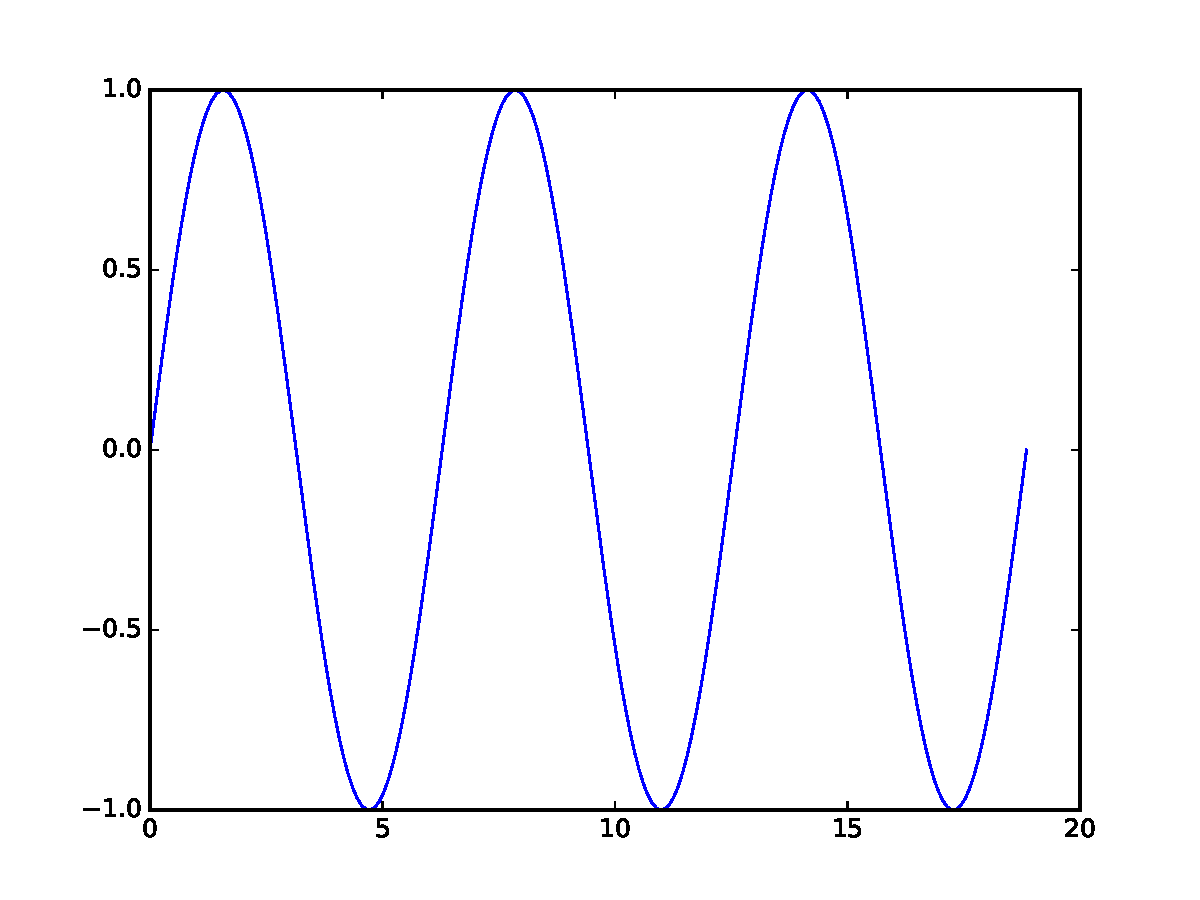
\includegraphics[width= \linewidth]{figures/exemplo_figure3_1.pdf}


\end{document}
